techniques\section{Results}
First we compare and contrast the performance of our jump points
pruning algorithm with the Swamps method of
\citeauthor{pochter10}~\shortcite{pochter10}. 
Both Swamps and jump points belong to the same family of methods:
optimality preserving pruning techniques for speeding up pathfinding.
When evaluating Swamps we used the authors'
source code and ran all experiments using their recommended running parameters:
a swamp seed radius of 6 and ``no change limit'' of 2. 
\par
Next, we compare and contrast the performance of jump points pruning 
against the HPA* algorithm of \citeauthor{botea04}~\shortcite{botea04}.
Though sub-optimal, HPA* is very fast and therefore widely applied in video
games. We compare against it to establish whether or not jump points are 
equally applicable in similar contexts. 
When evaluating HPA* we used a custom implementation of the algorithm and a
fixed cluster size of 10 (as recommended by the original authors).
\par
We discuss performance in terms of search times and compare 
the average speedup experienced by A* when running with and
without pruning methods applied to the map.  
Using this metric a speedup of 2.0 is twice as fast (higher is better).

\begin{figure*}[t]
   \begin{center}
	   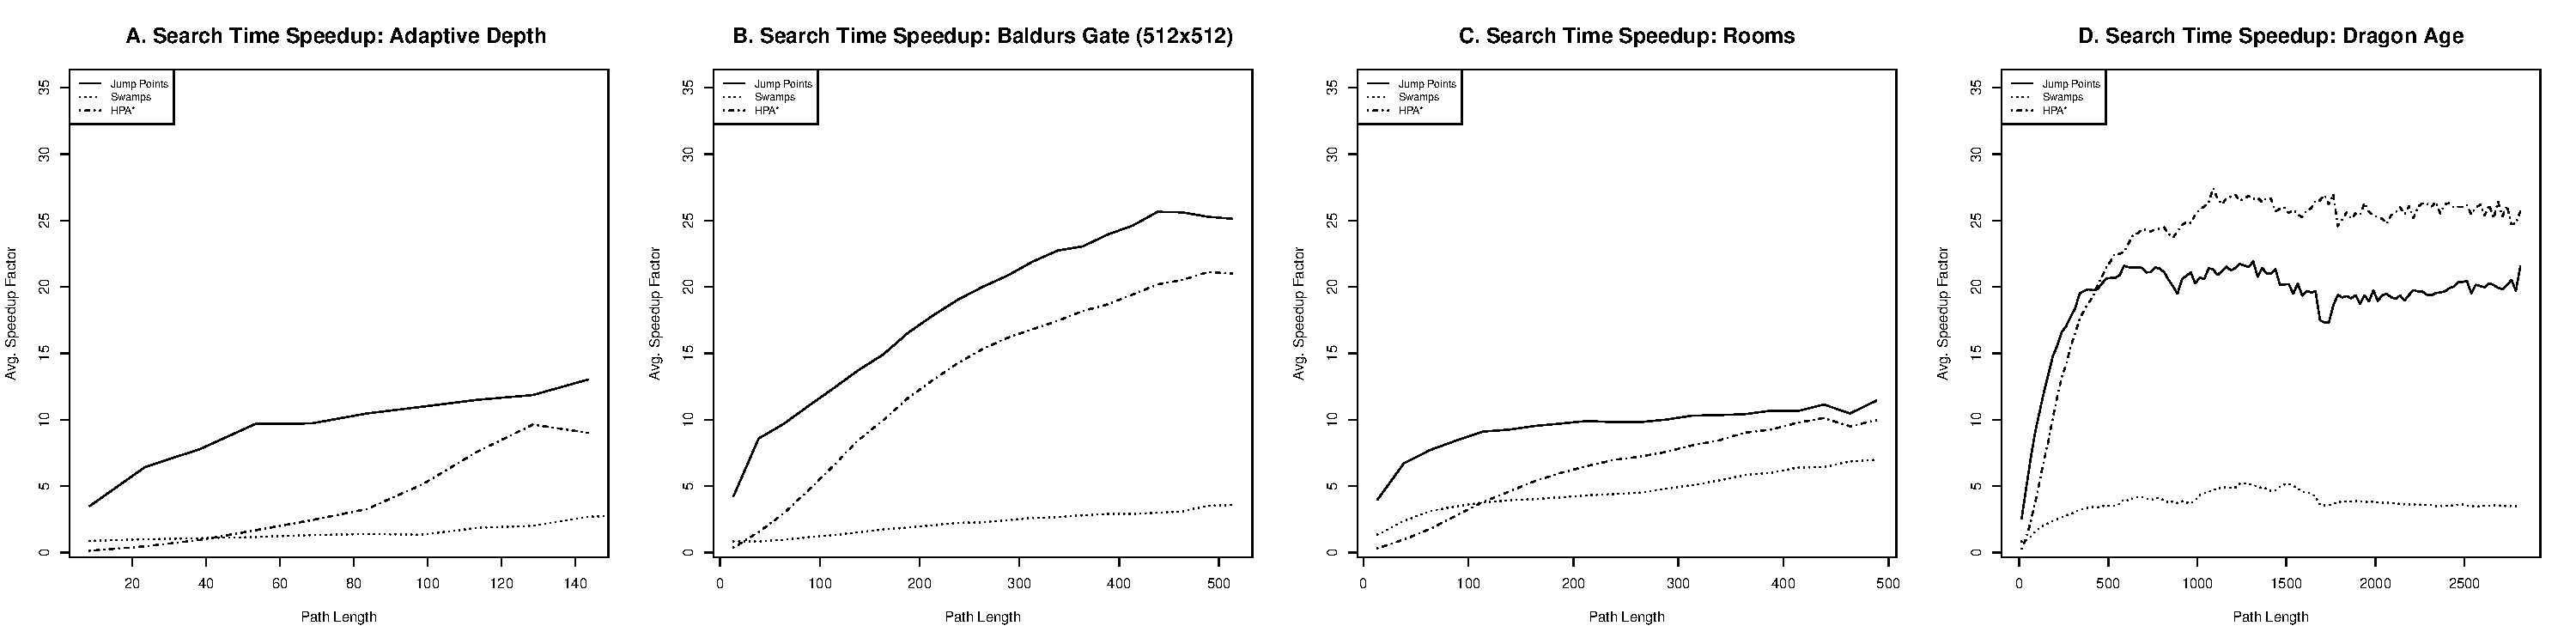
\includegraphics[width=2.0\columnwidth, trim = 10mm 10mm 10mm 0mm]
		{diagrams/speedup.pdf}
   \end{center}
   \caption{Average A* speedup on each of our four benchmarks. 
	Results are given in terms of relative search time improvement.}
\label{fig:speedup}
\end{figure*}

\textbf{Comparison with Swamps: }
As per Figure \ref{fig:speedup}(A-D), jump point pruning shows a convincing
improvement over Swamps across all benchmarks. 
The largest differences are observed on Baldur's Gate and Dragon Age where jump 
points achieve between 20-26 times search time speedup compared with Swamps with 
only attains a 3-5 times speedup.
On the Rooms benchmark the difference is much smaller: jump points pruning
speeds up search times by a factor of 11 while Swamps achieves a 7 times
speedup.
The observed performance characteristics are not unexpected: Swamps prune out
areas that can be avoided without introducing a detour. However, Swamps are of
little benefit if the areas which remain are large and need to be explored 
throroughly.
By comparison, jump points pruning rapidly explores large areas by proving
that many node expansion operations are unnecessary.
\textbf{Comparison with HPA*: }
$\ldots$
